%
%     卒業論文 (2004. 1)
%                         Authorized by Jun MUKAI
%
\documentclass[12pt]{jreport}
\usepackage{b_thesis}
\usepackage{ascmac}
\usepackage{deepsection}
\usepackage{drafts}
\usepackage[dvipdfmx]{graphicx, color}
\usepackage{here}
\usepackage{tabverb}
\usepackage{tabularx}
\usepackage{array}
\usepackage{moreverb}
\usepackage{fancybox}
\usepackage{comment}
\usepackage{algorithm}
\usepackage{algorithmic}
\usepackage{indentfirst}
\usepackage{multirow}
\usepackage{amsmath}

\pagestyle{headings}
%\pagestyle{drafts}

\topmargin=0.0truecm
\oddsidemargin=0.1truecm
\evensidemargin=0.1truecm
\textwidth=16cm
\textheight=22.5cm
\newcommand{\figurewidth}{14cm}

\title{行動情報と発話情報の組み合わせによる\\信念と欲求の逐次的推測モデルの検討}

\author{渡邊 悠太}                   % あなたのお名前
\teachera{今井 倫太 教授}
\teacherb{}
\teacherc{}
\authorname{渡邊 悠太}               % あなたのお名前
\date{}

\course{情報工学}
\id{61720736}                       % あなたの学籍番号

\begin{document}
\baselineskip = 20pt
\bibliographystyle{my_jalpha}
\nocite{*}
\maketitle                  %表紙がいらないときはコメントアウト

%
%     論文要旨
%
%
\jabst{
\hspace*{1zh}
\par
 本研究の目的は,人間にストレスを与えることの無い,使いやすい対話システムの実現である.単純な質問応答対話を超えた使いやすい対話システムを作るためには,対話相手に合わせて対話戦略を変えることが必要である.対話相手に合わせた対話を行うためには,人間の信念や欲求を推定することが重要である.人間の心的状態を推定する研究では,人間の散策行動から信念や欲求を推定する研究や人間の発話文から信念や欲求,意図を推定する研究がある.しかし既存研究では,
% 人間の散策行動情報と人間の発話情報の両方を用いて心的状態を推定する取り組みは少ないため,
人間の発話文による散策行動の解釈や散策行動による人間の発話の解釈を捉える方法は未だ確立されていない.本論文では,散策行動情報と人間の発話情報の両方を活用し,信念と欲求を逐次的に推定するシステムMultimodal Inference of Mind SCAIN (MIoM SCAIN)を提案する.MIoM SCAINは,散策行動情報と人間の発話情報の両方を活用して信念と欲求を推定することで,人間の発話内容による散策行動の解釈の決定や散策行動による人間の発話文の解釈を決定する.MIoM SCAINでは,独自に作成したデータセットを利用し推定システムを構築することで,人間の信念と欲求の推定を行うことができる.また,本論文では,散策行動情報と人間の発話情報の両方を活用した人間の信念と欲求の推定が有効であるかを評価する実験を行った.評価実験の結果,MIoM SCAINの推定性能が散策行動情報と人間の発話情報の一方のみから信念と欲求を推定するシステムの推定性能を上回り,散策行動情報と人間の発話情報の両方を活用した信念と欲求の推定が有効であることが示された.
}
\makejabstract
     %論文要旨
\newpage

\setcounter{page}{1}
\pagenumbering{roman}

\tableofcontents     %目次
\listoffigures       %図目次
\listoftables        %表目次
\newpage

\setcounter{page}{1}
\pagenumbering{arabic}

\baselineskip = 20pt




%%
%% 論文構成.ここは適宜変更する
%%
\chapter{序論}

\par
対話システムは,発話解釈と発話生成の両方において発展を遂げており,我々の生活に浸透しつつある.しかし人間は,対話システムとの対話において不自然さやストレスを感じることも少なくない.本研究の目的は,人間に不自然さやストレスを与えることが無い,使いやすい対話システムの実現である.

\par
対話システムと人間との対話では,対話システムが対話相手の心的状態を推定し,それを考慮した対話を行うことが重要である.
人間は,気分が落ち込んでいる対話相手の発話に対してネガティブな発話解釈をしたり,励ましの言葉をかけるように,対話相手の心的状態によって相手の発話の解釈を変えたり,自身の発話の内容を変えている.また,相手が知らないことについて詳しく説明したり,相手が好むことについて話を掘り下げる.対話システムにおいても,人間と同様に対話相手の心的状態に合わせて,発話解釈を変えたり,自身の発話の内容を変えることで,より自然でありストレスの少ない対話を実現することができる.つまり,対話相手に合わせた臨機応変な発話解釈や発話生成により対話における不自然さやストレスをなくすためには,対話相手の心的状態を推定することが必要となる.


\par
人間の心的状態を推定する研究には,人間の散策行動情報から心的状態を推定する研究や発話情報から心的状態を推定する研究が存在する.人間の散策行動情報から心的状態を推定する研究は,代表的には,環境の状態と環境中を移動する人間の散策行動や観測状況をベイズ推定\cite{alma9926464316904034}に適用し,環境中を移動する人間の信念と欲求を推定する研究 \cite{baker2011bayesian}があげられる.信念はどのようなことを考えているかということを意味し,欲求は何を望んでいるかということを意味する.発話情報から心的状態を推定する研究では,代表的には,人間の発話情報から得られた事象を信念と捉え,考えられる欲求の候補を生成し,尤もらしい欲求を基に発話者の意図を推定する研究 \cite{高橋拓誠2015bdi}があげられる.また,ユーザの信念,欲求および意図を考慮することによる検索精度の向上のために検索クエリへの入力から人間の信念,欲求および意図を推定する研究 \cite{10.1007/978-3-642-02481-8_4}や,機械翻訳において,ユーザの信念によって翻訳の粒度や表現を変えるために,入力文からユーザの信念を推定する研究\cite{farwell1997user}も存在する.

% 教師の発話から学習者の心的状態を推定する

\par
従来研究では,散策行動情報のみから人間の信念と欲求を推定する研究や人間の発話情報のみから人間の信念と欲求を推定する研究は存在した.しかし,散策行動情報と人間の発話情報の両方を活用し人間の信念と欲求を推定する取り組みは少ない.従来研究における信念と欲求の推定は,遠くから散策行動を観測している場合や立ち止まって対話をしている場合というように,散策行動情報のみが観測される場合や人間の発話情報のみが観測される場合には有効である.しかし実世界では,散策行動情報と人間の発話情報の両方が観測されることが多く,人間の発話情報によって散策行動情報の解釈が依存して決まったり,散策行動情報によって人間の発話情報の解釈が依存して決まることがある.
\begin{figure}[htbp]
  \begin{center}
    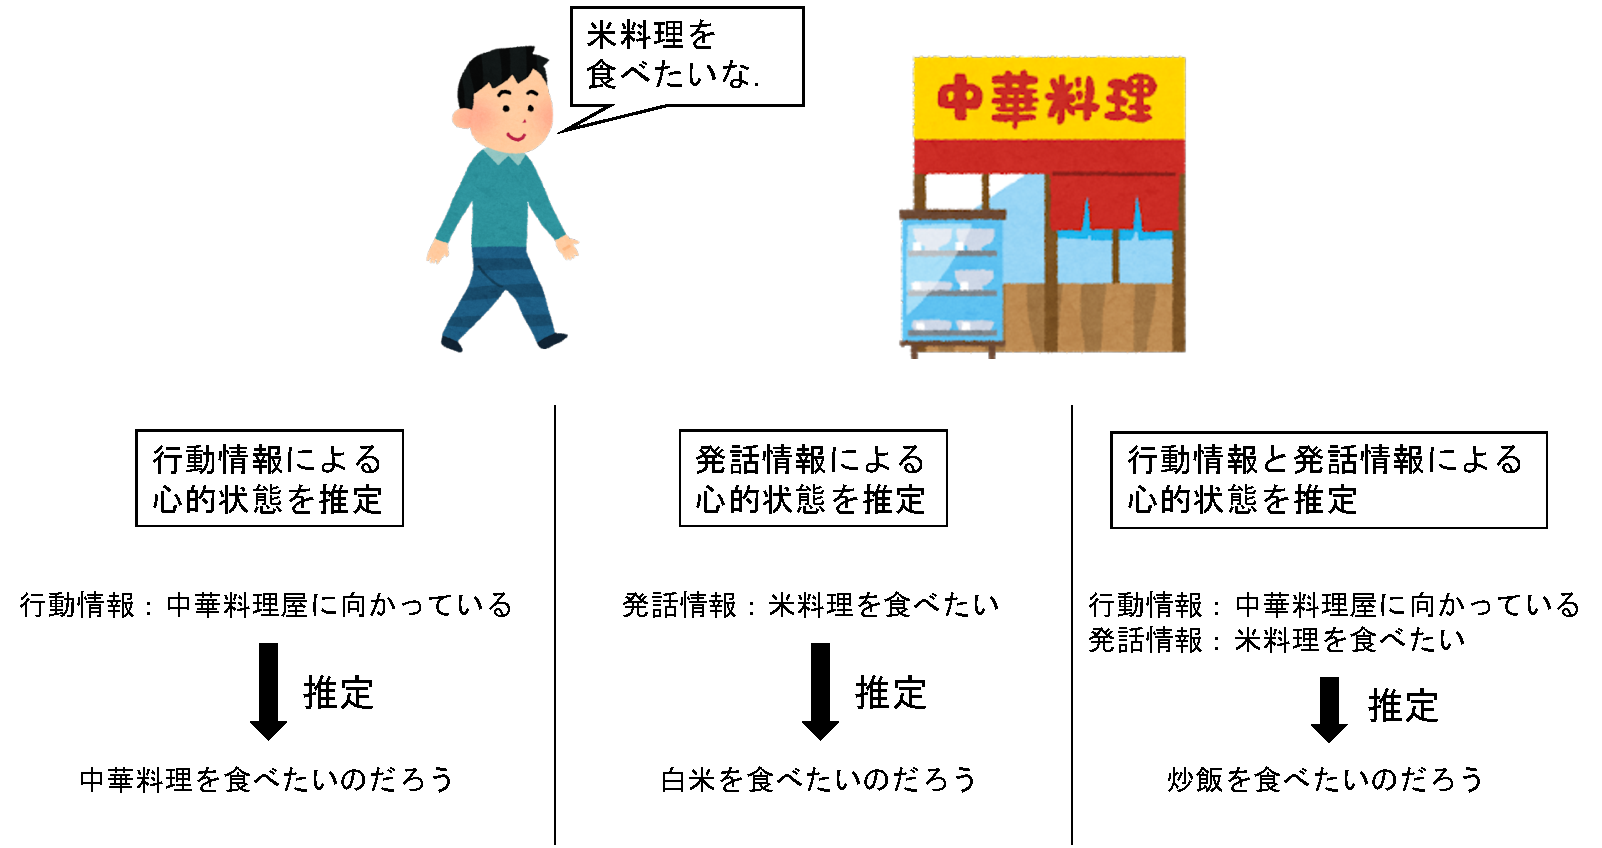
\includegraphics[scale=0.5]{./figure1.pdf}
    \caption{散策行動情報と人間の発話情報の相互作用を考慮した信念と欲求の推定}
    \label{fig:fig1}
  \end{center}
\end{figure}
例えば,図\ref{fig:fig1}の左側の状況において,散策行動情報は「料亭と中華料理屋が並ぶ飲食店街に向かっている」と解釈できるが,図\ref{fig:fig1}の右側の状況のように「魚料理を食べたいな」という人間の発話情報が観測された時,散策行動情報は「料亭に向かっている」と解釈される.
従来研究では,散策行動情報と人間の発話情報の両方が観測される場合においては,人間の発話情報による散策行動情報の解釈の決定や,散策行動情報による人間の発話情報の解釈の決定をすることが難しい.つまり,散策行動と人間の発話の両方が観測される場合における従来研究における信念と欲求の推定では,散策行動と人間の発話の相互依存の考慮による推定性能の向上の可能性が低いことが予想される.
% 従来研究では,行動情報のみから人間の心的状態を推定する研究や発話情報のみから人間の心的状態を推定する研究は存在した.しかし,行動情報と発話情報の両方を活用し人間の心的状態を推定する研究はない.従来研究における心的状態の推定は,遠くから行動を観測している場合や立ち止まって対話をしている場合というように,行動情報のみが観測される場合や発話情報のみが観測される場合には有効である.しかし実世界では,図\ref{fig:fig1}にように行動情報と発話情報の両方が観測されることが多く,発話情報によって行動情報の解釈が変わったり,行動情報によって発話情報の解釈が変わることがある.
% \begin{figure}[htbp]
%   \begin{center}
%     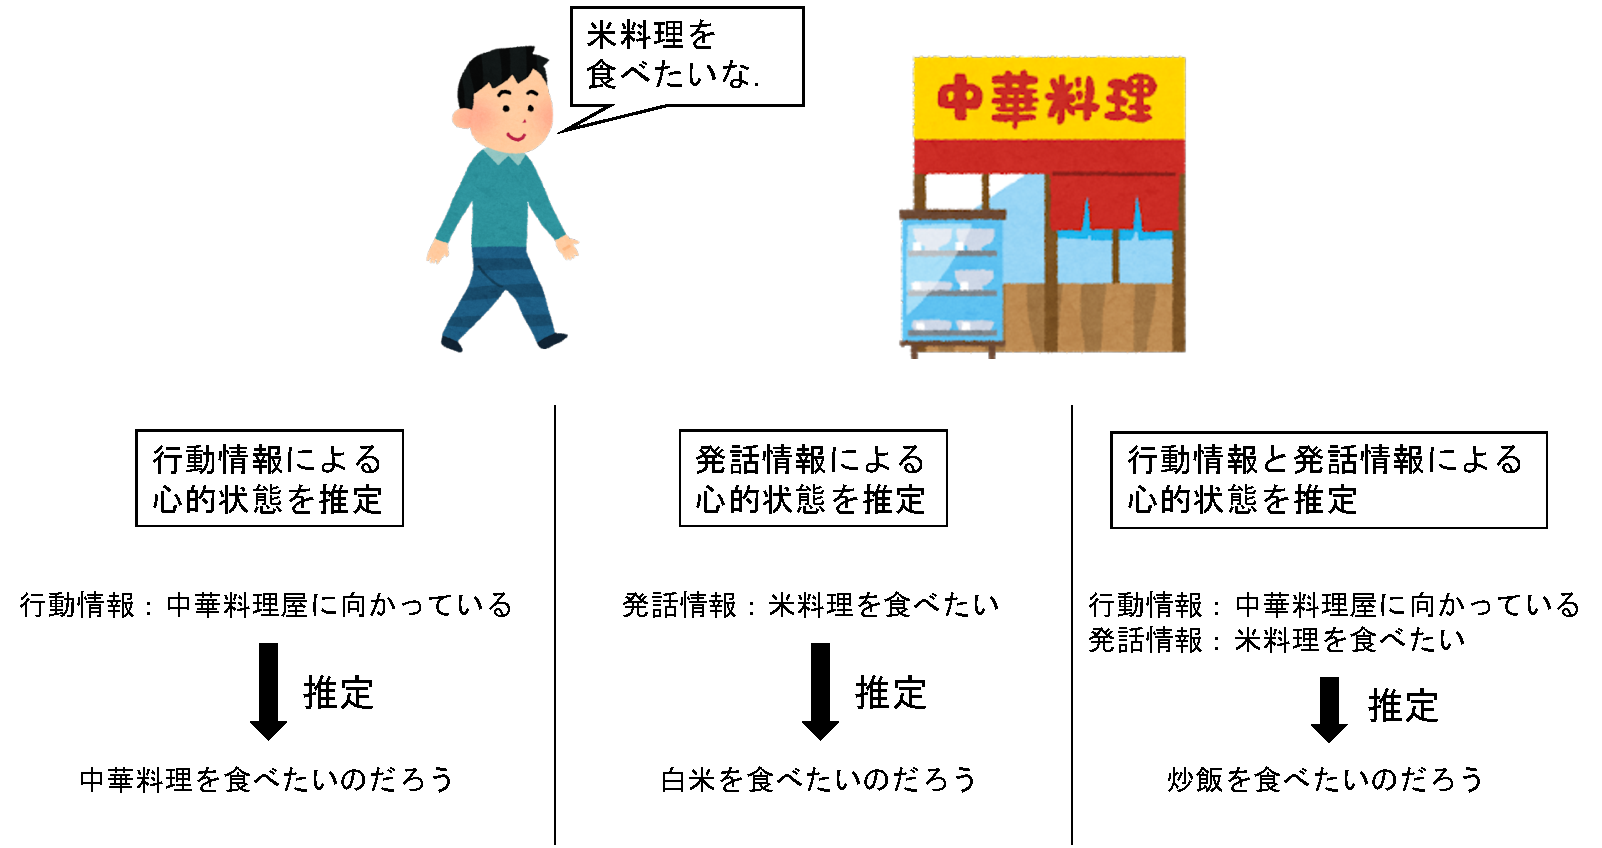
\includegraphics[scale=0.58]{./figure1.pdf}
%     \caption{心的状態の推定.人間が食事をとるために飲食店に向かう場面において,3通りの条件で心的状態を推定する.図の左側は,行動情報のみを活用して心的状態を推定した場合,図の中央は発話情報のみを活用して心的状態を推定した場合,図の右側は行動情報と発話情報の両方を活用して心的状態を推定した場合を表す.}
%     \label{fig:fig1}
%   \end{center}
% \end{figure}
% また行動情報のみを活用して「中華料理を食べたいのだろう」という心的状態を推定したり発話情報のみを活用して「白米を食べたいのだろう」という心的状態を推定するのに対し,行動情報と発話情報の両方を活用して「炒飯を食べたいのだろう」という心的状態を推定するように,行動情報と発話情報の両方を活用することにより,発話情報による行動情報の解釈の変化や行動情報による発話情報の解釈の変化を捉えることが可能となり,より多くの情報を基に推定を行うことができる.
% 従来研究では,行動情報と発話情報の両方が観測される場合においては,発話情報による行動情報の解釈の変化や,行動情報による発話情報の解釈の変化を捉えることが難しい.つまり,行動と発話の両方が観測される場合における従来研究における心的状態の推定では,行動と発話の相互作用の考慮による推定性能の向上の可能性が低いことが予想される.

\par
本研究では,散策行動情報と人間の発話情報の両方から人間の心的状態の一部である信念および欲求を逐次的に推定するシステムMultimodal Inference of Mind SCAIN (MIoM SCAIN)を提案する.MIoM SCAINは,人間の信念および欲求の推定において,信念と欲求の組み合わせをを一つに断定するのではなく,同時に複数保持し,やり取りの中で動的に推定する.MIoM SCAINは,散策行動情報と人間の発話情報の両方を推定に活用し,ベイズ推定によって人間の信念および欲求を逐次的に推定する.散策行動情報と人間の発話情報の両方を推定に活用することにより,図\ref{fig:fig1}の右側の状況における推定のように,人間の発話情報による散策行動情報の解釈の決定や散策行動情報による人間の発話情報の解釈を決定を行い,散策行動情報と人間の発話情報の相互依存を考慮した推定が可能となる.実験では,独自で作成したデータセットを利用し,MIoM SCAINにより信念と欲求の推定を行い,散策行動情報と人間の発話情報の両方を推定に活用することが有効であるかを評価する.

\par
本論文の構成は以下の通りである.第二章では,関連研究においてどのように人間の信念や欲求を推定していたかを述べる.第三章では,人間の散策行動情報と人間の発話情報から信念と欲求を推定するシステムMIoM SCAINを提案する.第四章では,MIoM SCAINと散策行動情報もしくは人間の発話情報のみから信念と欲求を推定するシステムを用いて実験的に評価し,第五章では評価結果について考察する.第六章では,MIoM SCAINにおける今後の課題について述べる.最後に,第七章で本論文を締めくくる.

\chapter{関連研究}
\section{行動情報から心的状態を推定する研究}


\section{発話情報から心的状態を推定する研究}


\section{単一情報による心的状態推定の問題点}

\chapter{提案}
\par
本論文では,行動情報と発話情報の両方を活用する心的状態推定システムMultimodal Inference of Mind(MIoM)を提案する.MIoMは,人間の信念や行動,発話および人間が存在する環境の状態を基に心的状態を推定する.行動情報と発話情報の両方を心的状態の推定に活用することで,発話による行動の解釈の変化や行動による発話に解釈の変化を捉え,行動情報と発話情報の相互作用を考慮して心的状態を推定する.

\par
MIoMは,環境の状態や人間の心的状態を部分的に観測可能なマルコフ決定過程(POMDP)として表される.また,心的状態とその尤度を持つパーティクルフィルタとして表され,心的状態を一意に決め付けるのではなく同時に複数保持し,時刻が経過する度に各パーティクルの尤度を更新していく.各時刻おける人間の信念や行動,発話および人間が存在する環境の状態をベイズの定理に適用し,人間が観測できていない環境領域についての信念と欲求を逐次的に推定する.


\section{関連研究との相違点}
\par
MIoMと関連研究との相違点は,行動情報と発話情報の両方を活用したマルチモーダルな心的状態推定を行う点である.MIoMは,行動情報と発話情報の両方を活用して心的状態を推定することで,発話による行動の解釈の変化や行動による発話の解釈の変化を捉え,行動情報と発話情報の相互作用を考慮した推定が可能となる.MIoMは,関連研究における問題点を解消するシステムとなっている.


\section{アルゴリズム}

\par
MIoMにおける推定処理の流れをを図\ref{fig:sys_arc}に示す.
\begin{figure}[htbp]
  \begin{center}
    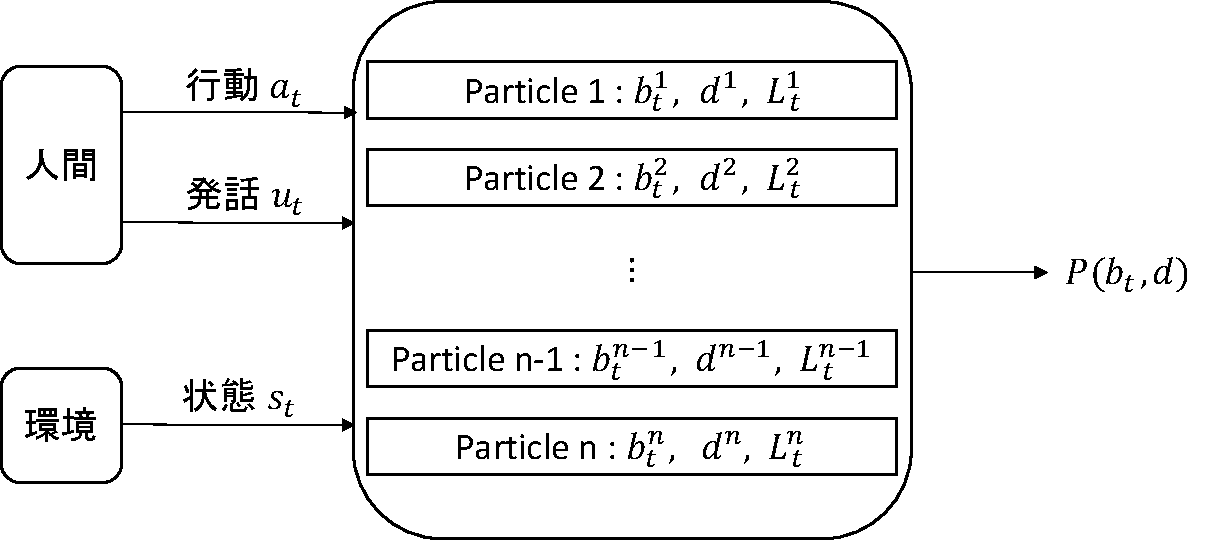
\includegraphics[scale=0.75]{./bt1.pdf}
    \caption{MIoMによる推定処理}
    \label{fig:sys_arc}
  \end{center}
\end{figure}
図\ref{fig:sys_arc}に示すように,MIoMは時刻$t$における人間の行動$a_t$,発話$u_t$および環境の状態$s_t$から信念と欲求の確率を出力する.MIoMは信念$b_t$と欲求$d$の組み合わせとその尤度$L$を持つパーティクルフィルタとして表現され,$a_t,u_t,s_t$を基にそれぞれのパーティクルの尤度$L^k$が更新される.ここで,尤度$L^k$は次のように表すことができる.
\begin{equation}
  \begin{split}
  \label{pf}
  L^k=P(b_t^k,d^k|s_{1:t},a_{1:t-1},u_{1:t-1})
  \end{split}
\end{equation}
ここで,$u_{1:t-1}$は,時刻$1$から時刻$t-1$までの人間の発話履歴,$P(b_t,d|s_{1:t},a_{1:t-1},u_{1:t-1})$は,$s_{1:t},a_{1:t-1}およびu_{1:t-1}$から計算される$b_t$と$d$の確率である.

\par
図\ref{fig:miom}にMIoMにおけるベイズ推論の様子を示す.
\begin{figure}[htbp]
  \begin{center}
    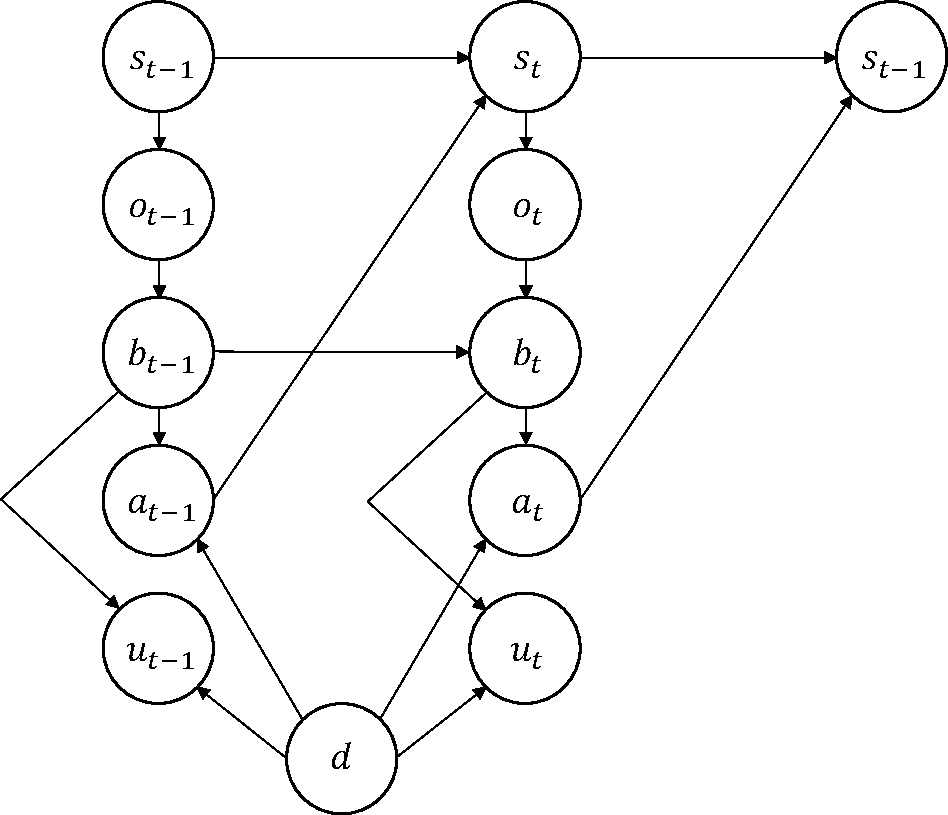
\includegraphics[scale=0.85]{./miom.pdf}
    \caption{MIoMにおけるベイズ推定}
    \label{fig:miom}
  \end{center}
\end{figure}
MIoMにおけるベイズ推論では,BToMと同様に時刻$t$における環境の状態$s_{t}$を基に人間の観測状況$o_{t}$が決まる.また,$o_{t}$を基に人間の信念$b_{t}$が決まり,$b_{t}$と人間の欲求$d$から人間の行動$a_{t}$が決まる.それに加え,MIoMでは$b_t$と$d$から人間の発話$u_t$が決まる.また$a_{t}$起こることにより,環境の状態は$s_{t+1}$に変化し,人間の観測状況,信念,行動および発話が再起的に決定される.MIoMでは各パーティクルの尤度である式(\ref{pf})を計算することを目的としている.以下に,式(\ref{pf})にベイズの定理を適用した過程を示す.

\begin{equation}
  \begin{split}
  \label{eq_miom}
  L^k&=P(b_t^k,d^k|s_{1:t},a_{1:t-1},u_{1:t-1})\\
  &\propto P(b_t^k,d^k,s_{1:t},a_{1:t-1},u_{1:t-1})\\
  &= \sum_{b_{t-1}^k,o_t}P(b_t^k,d^k,s_{1:t},a_{1:t-1},u_{1:t-1},b_{t-1}^k,o_t)\\
  &= \sum_{b_{t-1}^k,o_t}P(b_t^k|d^k,s_{1:t},a_{1:t-1},u_{1:t-1},b_{t-1}^k,o_t)\cdot P(d^k,s_{1:t},a_{1:t-1},u_{1:t-1},b_{t-1}^k,o_t)\\
  &= \sum_{b_{t-1}^k,o_t}P(b_t^k|b_{t-1}^k,o_t)\cdot P(o_t|d^k,s_{1:t},a_{1:t-1},u_{1:t-1},b_{t-1}^k)\\
  &\hspace{5cm} \cdot P(d^k,s_{1:t},a_{1:t-1},u_{1:t-1},b_{t-1}^k)\\
  &= \sum_{b_{t-1}^k,o_t}P(b_t^k|b_{t-1}^k,o_t)\cdot P(o_t|s_t)\cdot P(s_t|s_{t-1},a_{t-1})\\
  &\hspace{3cm} \cdot P(a_{t-1}|b_{t-1}^k,d^k)\cdot P(u_{t-1}|b_{t-1}^k,d^k)\cdot P(b_{t-1}^k,d^k,s_{t-1},a_{t-2},u_{t-2})\\
  \end{split}
\end{equation}


ここで,$P(b_t^k|b_{t-1}^k,o_t)$は人間の観測$o_t$によって$k$番目のパーティクルの信念$b_t^k$が更新される確率,$P(o_t|s_t)$は環境の状態$s_t$において人間が観測状況$o_t$を得る確率,$P(s_t|s_{t-1},a_{t-1})$は環境の状態$s_{t-1}$において人間が行動$a_{t-1}$を起こした時に環境の状態が$s_{t}$になる確率,$P(a_{t-1}|b_{t-1}^k,d^k)$は$k$番目のパーティクルが信念$b_{t-1}^k$,欲求$d^k$を持っている時に行動$a_{t-1}$を起こす確率,$P(u_{t-1}|b_{t-1}^k,d^k)$は$k$番目のパーティクルが信念$b_{t-1}^k$,欲求$d^k$を持っている時に発話$u_t$を起こす確率,$P(b_{t-1}^k,d^k,s_{t-1},a_{t-2},u_{t-2})$は時刻$t-1$における$k$番目のパーティクルの尤度である.式(\ref{eq_miom})より,$L^k$は再起関数として表すことができ,初期値$P(b_1,d,s_1,a_0,u_0)$を決めることで更新することができる.また,$P(b_t^k|b_{t-1}^k,o_t)$,$P(o_t|s_t)$,$P(s_t|s_{t-1},a_{t-1})$,$P(a_{t-1}|b_{t-1}^k,d^k)$および$(u_{t-1}|b_{t-1}^k,d^k)$の乗算として表すことができる.

\par
% それぞれの生起確率がどのように計算されるかを記載
MIoMでは,各時刻における$P(b_t^k|b_{t-1}^k,o_t)$,$P(o_t|s_t)$,$P(s_t|s_{t-1},a_{t-1})$,$P(a_{t-1}|b_{t-1}^k,d^k)$および$(u_{t-1}|b_{t-1}^k,d^k)$を計算し,乗算することで,その時刻における信念と欲求の尤度を計算する.$P(b_t^k|b_{t-1}^k,o_t)$は既に人間が$b_t^k$を観測しているかどうかを$o_t$によって計算する.
$P(a_{t-1}|b_{t-1}^k,d^k)$は信念$b_{t-1}^k$と欲求$d^k$を基に上,下,左,右の4方向の確率を計算する.$(u_{t-1}|b_{t-1}^k,d^k)$はWord2Vecにより発話$u_t$を分散表現に変換した後,信念$b_{t-1}^k$と欲求$d^k$との類似度を基に計算する.

\chapter{評価}
\par
行動情報と発話情報の両方を反映した信念と欲求の推定が有効であることを示すため,MIoM SCAINと単一情報による信念と欲求の推定システムUnimodal Inference of Mind SCAIN (UIoM SCAIN)の推定精度を比較する.行動情報と発話情報には,本研究で作成したデータセットを利用する.


\section{実験設定}
\par
BToMによる信念および欲求の推定を評価するための実験を参考に,学生がアシストロボットとともに屋台で食事を買うシーンを想定する.図\ref{fig:ex_env1}に本実験における環境の一例を示す.
\begin{figure}[htbp]
  \begin{center}
    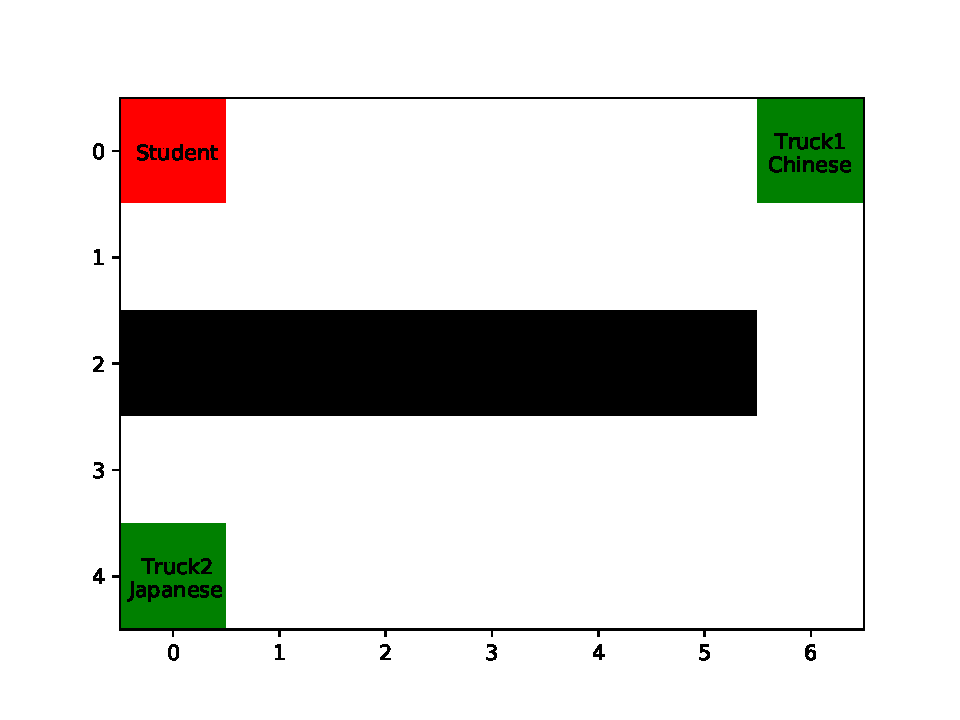
\includegraphics[scale=0.7]{./ex_env1.pdf}
    \caption{本実験における環境.図中の``Student''は学生,``Truck1''および``Truck2''は屋台を開くスペース,中央の黒色部分は壁を表す.}
    \label{fig:ex_env1}
  \end{center}
\end{figure}
7$\times$5マスで表現される環境中に壁とTruck1およびTruck2で表される屋台を開くスペースが存在し,それぞれのスペースに日本食の屋台,イタリア料理の屋台,中華料理の屋台のいずれかが出店する.環境中の学生は移動し,アシストロボットと対話をしながら食事を購入する屋台を決める状況を考える.学生は,日本食の屋台,イタリア料理の屋台,中華料理の屋台の3種類のうち2種類が出店することは知っているが,どの屋台が出店しているかは知らないため,環境中を移動しアシストロボットと対話しながら食事を買う屋台を選ぶ.学生の行動$a_t$は上,下,左,右の4方向への移動とし,発話$u_t$はアシストロボットから提示される食事に関する質問に対する学生の応答とする.信念$b_t$は,壁により観測できていない屋台に関してどの屋台が出店していると考えているか,欲求$d$は学生が3種類のそれぞれの屋台をどの程度好むかを表す.



\section{実験手順}

\par
本実験には,本研究で作成したデータセットを利用した.本データセットには,屋台の組み合わせを表す環境設定と,その環境設定で考えられる学生の行動,アシストロボットからの質問,学生の応答が含まれる.屋台の組み合わせは日本食の屋台,イタリア料理の屋台,中華料理の屋台の2つの組み合わせとする6通り,学生の行動は上,下,左,右の4方向への移動,アシストロボットからの質問は表\ref{tab:q_a}の左側に記載される4通り,学生の応答は表\ref{tab:q_a}の右側に記載される8通りである.
\begin{table}[htb]
  \begin{center}
  \caption{アシストロボットからの質問と学生の応答}
  \label{tab:q_a}
  \begin{tabular}{lll} \hline
    質問内容&\multicolumn{2}{l}{応答内容}\\\hline
    魚料理と野菜料理どちらを食べたいですか&fish&vegetable\\
    パスタと米ではどちらを食べたいですか&pasta&rice\\
    あっさりしたものと,こってりしたものどちらを食べたいですか&plain&oily\\
    辛いものと酸っぱいものではどちらを食べたいですか&spicy&sour\\\hline
  \end{tabular}
\end{center}
\end{table}
本実験では,一定時間パーティクルの尤度に大きな変化がない時およびTruck1を通り過ぎた時に質問を提示した.MIoM SCAINによって行動情報と発話情報の両方を信念と欲求の推定に活用することが有効であることを評価するために,パーティクルフィルタを用い行動情報と発話情報の一方のみを基に信念と欲求を推定するシステムUnimodal Inference of Mind SCAIN (UIoM SCAIN)を定義した.


\par
図\ref{fig:interface}に示すインターフェスを用いて,30人の実験参加者に,本データセットで指定された環境設定と行動およびアシストロボットからの質問と学生の応答を提示し,環境中の学生の信念と欲求をそれぞれ7段階で推定させた.
\begin{figure}[htbp]
  \begin{center}
    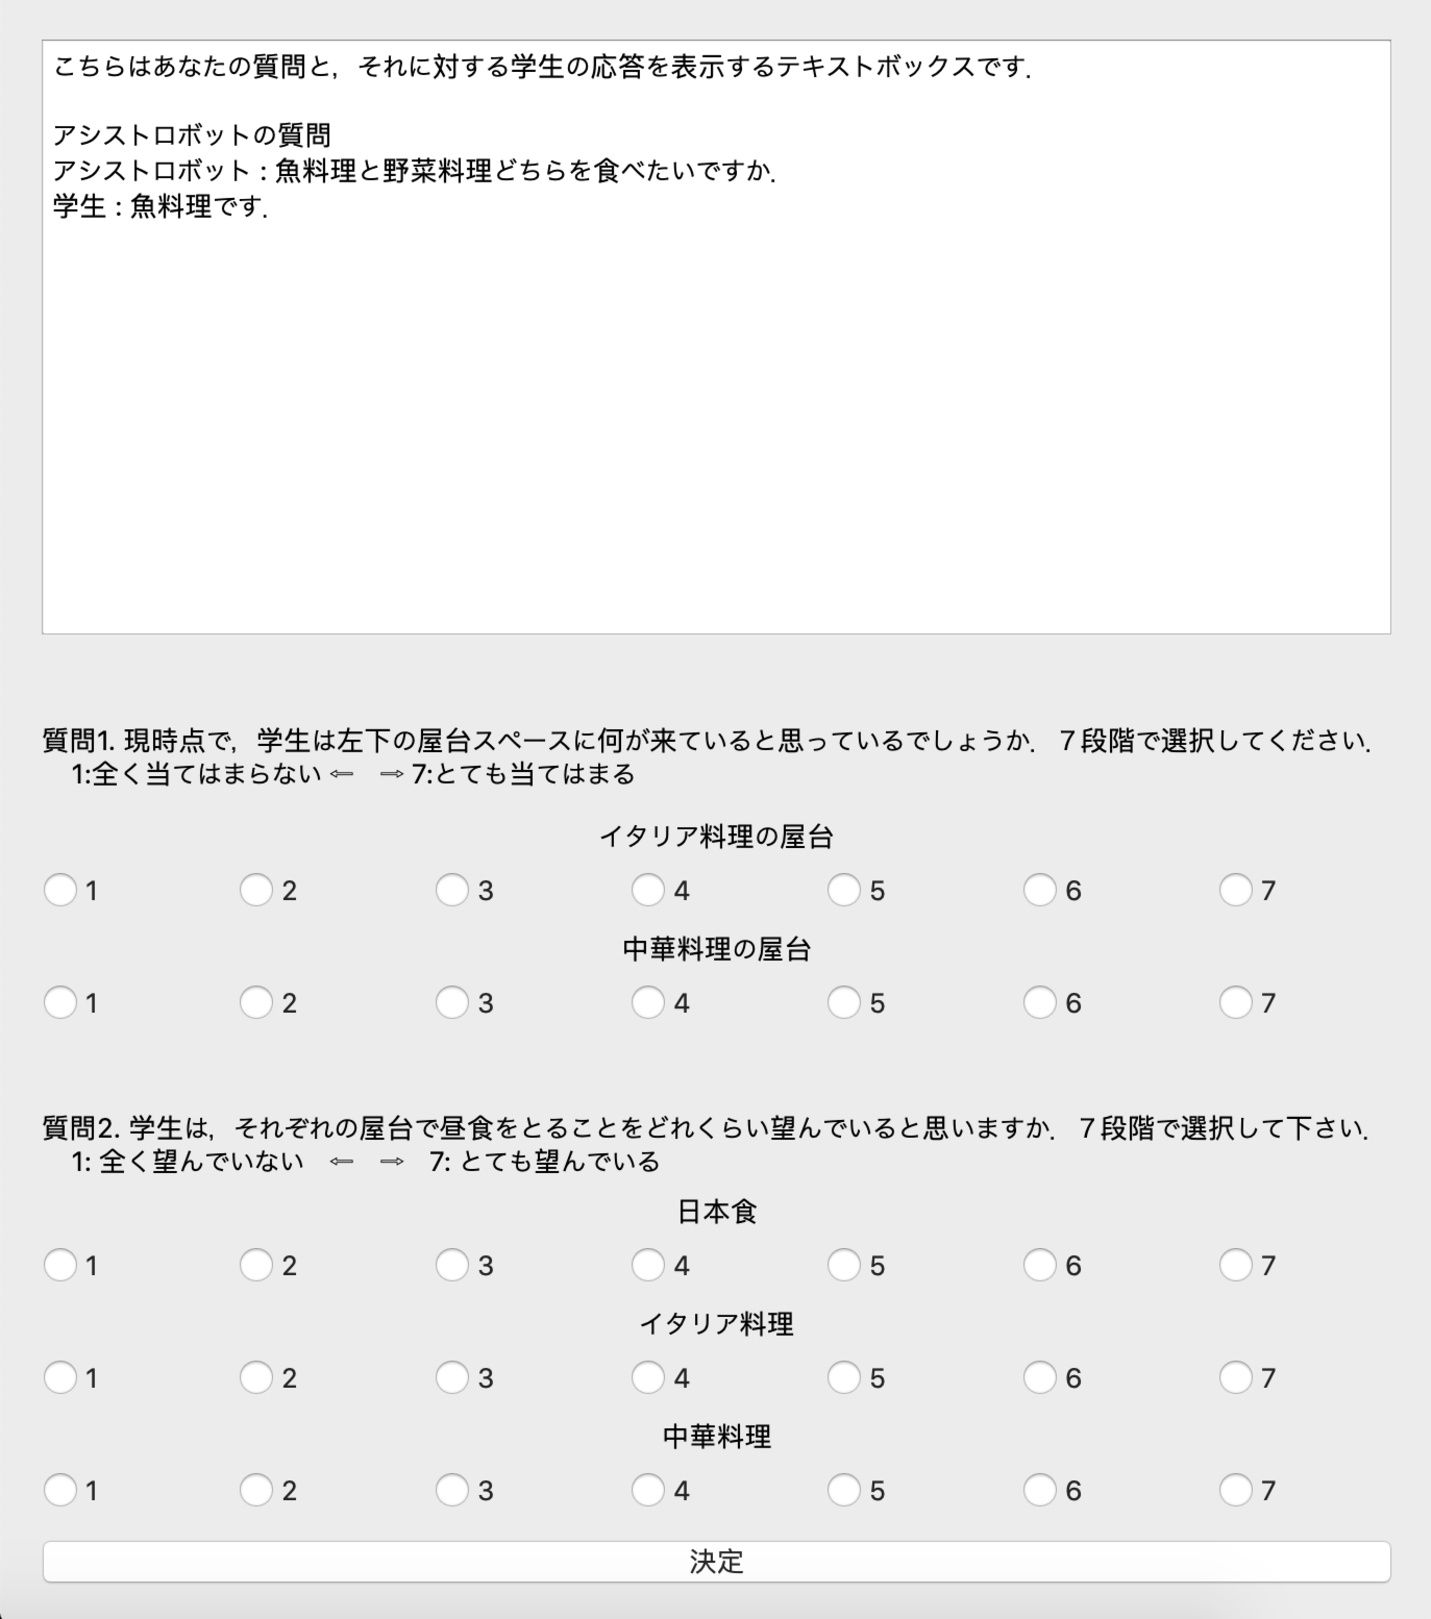
\includegraphics[scale=0.6]{./interface.pdf}
    \caption{本実験に使用したインターフェース}
    \label{fig:interface}
  \end{center}
\end{figure}
環境設定や行動の内容,アシストロボットからの質問,学生の応答に偏りがないように8つのデータを本データセットから選択し,それぞれの実験参加者に対して提示し,1つのデータに対して2回または3回推定をさせた.
また,MIoM SCAIN (action + utterance),行動情報のみを基に心的状態を推定するUIoM SCAIN (action),発話情報のみを基に心的状態を推定するUIoM SCAIN (utterance)の3つのシステムによって,環境中の学生の信念と欲求を推定し,推定結果を式(\ref{b_transform})および式(\ref{d_transform})により,7段階評価に変換した.
\begin{equation}
  \begin{split}
  \label{b_transform}
  b_t(\mathrm{Japanese})= \sum_{\substack{k\\b_t^k=\mathrm{Japanese}}} 7\cdot L^k\\
  b_t(\mathrm{Italian})=\sum_{\substack{k\\b_t^k=\mathrm{Italian}}} 7\cdot L^k\\
  b_t(\mathrm{Chinese})=\sum_{\substack{k\\b_t^k=\mathrm{Chinese}}} 7\cdot L^k\\
  \end{split}
\end{equation}

\begin{equation}
  \begin{split}
  \label{d_transform}
  d(\mathrm{Japanese})= \sum_{\substack{k\\d^k=\mathrm{Japanese}}} \frac{7}{3}\cdot L^k \cdot rank^k({\mathrm{Japanese}})\\
  d(\mathrm{Italian})= \sum_{\substack{k\\d^k=\mathrm{Italian}}} \frac{7}{3}\cdot L^k \cdot rank^k({\mathrm{Italian}})\\
  d(\mathrm{Chinese})= \sum_{\substack{k\\d^k=\mathrm{Chinese}}} \frac{7}{3}\cdot L^k \cdot rank^k({\mathrm{Chinese}})\\
  \end{split}
\end{equation}
ここで,$rank^k(\mathrm{food})$は,パーティクル$k$における欲求$d_k$を基に$\mathrm{food}$をどの程度好むかを3段階で表した値である.式(\ref{b_transform})および式(\ref{d_transform})において,尤度が最大のパーティクルのみを用いて信念や欲求を推定することをせずに,全てのパーティクルを考慮して計算を行っているのは,各パーティクルの尤度に差がない場合に対応するためである.推定を行った全タイミングで,信念推定および欲求推定のそれぞれについて,実験参加者による推定結果とMIoM SCAINおよびUIoM SCAINによる推定結果を比較し,相関係数を算出した.UIoM SCAIN (action)およびUIoM SCAIN (utterance)の尤度は,それぞれ式(\ref{uiom_a}),式(\ref{uiom_u})で計算した.それぞれのモデルについて,信念または欲求の推定において相関係数が最大になるように,式(\ref{calc_a})における$cost$の計算に用いる報酬や,式(\ref{calc_u})における関数similarity内のパラメータを設定した.
\begin{equation}
  \begin{split}
  \label{uiom_a}
  L^k({\mathrm{action}})&= \sum_{b_{t-1}^k,o_t}P(b_t^k|b_{t-1}^k,o_t)\cdot P(o_t|s_t)\cdot P(s_t|s_{t-1},a_{t-1})\\
  &\hspace{3cm}\cdot P(a_{t-1}|b_{t-1}^k,d^k)\cdot P(b_{t-1}^k,d^k,s_{t-1},a_{t-2})
  \end{split}
\end{equation}

\begin{equation}
  \begin{split}
  \label{uiom_u}
  L^k({\mathrm{utterance}})&= \sum_{b_{t-1}^k,o_t}P(b_t^k|b_{t-1}^k,o_t)\cdot P(o_t|s_t)\cdot P(s_t|s_{t-1},a_{t-1})\\
  &\hspace{3cm}\cdot P(u_{t-1}|b_{t-1}^k,d^k)\cdot P(b_{t-1}^k,d^k,s_{t-1},u_{t-2})
  \end{split}
\end{equation}


\section{実験結果}

\par
表\ref{tab:cof}に,実験参加者による信念と欲求の推定結果とUIoM SCAIN (action), UIoM SCAIN (utterance)およびMIoM SCAINによる信念と欲求の推定結果との間の相関係数を示す.
\begin{table}[htb]
  \begin{center}
  \caption{人間による推定と推定モデルの相関}
  \label{tab:cof}
  \begin{tabular}{lcc} \hline
    \multirow{2}{*}{モデル}&\multicolumn{2}{c}{相関}\\\cline{2-3}
    & \hspace{10pt} 信念 \hspace{10pt} & \hspace{10pt} 欲求 \hspace{10pt} \\ \hline
    UIoM SCAIN (action)&0.124&0.419\\
    UIoM SCAIN (utterance)&0.216&0.494\\
    MIoM SCAIN (action + utterance)&\bf0.244&\bf0.550 \\\hline
  \end{tabular}
\end{center}
\end{table}


\par
表\ref{tab:cof}より,いずれの推定システムにおいても欲求推定の相関が信念推定の相関よりも強いことがわかった.

\par
また,信念と欲求の推定の両方において,行動情報と発話情報の両方を推定に活用するMIoM SCAINが行動情報のみを推定に活用するUIoM SCAIN (action)および発話情報のみを推定に活用するUIoM SCAIN (utterance)よりも強い相関を示すことがわかった.

\par
ここで,MIoM SCAINによる信念と欲求の推定の相関とUIoM SCAINによる信念と欲求の推定の相関との間に差があると言えるかを$z$検定\cite{alma9926301497204034}によって検定した過程を示す.また,表\ref{tab:test}に検定結果を示す.

\par
まず,MIoM SCAINとUIoM SCAIN (action)の信念推定における相関に差があるかを調べる.以下のように仮説を設定する.
\begin{displaymath}
  \begin{split}
  \label{z_a_b_p}
  \mathrm{帰無仮説:MIoM\; SCAINとUIoM\; SCAIN\; (action)の信念推定の相関に差がない}\\
  \mathrm{対立仮説:MIoM\; SCAINとUIoM\; SCAIN\; (action)の信念推定の相関に差がある}\\
  \end{split}
\end{displaymath}
また,データ数を考慮して検定統計量$T$は以下のように計算される.
\begin{displaymath}
  \begin{split}
  \label{z_a_b}
  T&=\sqrt{960-3}\left(\frac{1}{2}\ln{\frac{1+0.244}{1-0.244}-\frac{1}{2}\ln{\frac{1+0.124}{1-0.124}}}\right)\\
  &=3.85\\
  \end{split}
\end{displaymath}
$\alpha=0.05$で両側検定を行う.$z\left(\frac{\alpha}{2}\right)=1.96$であり,$T=3.85>1.96$なので,帰無仮説を棄却する.よって,MIoM SCAINとUIoM SCAIN (action)の信念推定における相関に差があると言える.

\par
次に,MIoM SCAINとUIoM SCAIN (utterance)の信念推定における相関に差があるかを調べる.以下のように仮説を設定する.
\begin{displaymath}
  \begin{split}
    \label{z_a_b}
    \mathrm{帰無仮説:MIoM\; SCAINとUIoM\; SCAIN\; (utterance)の信念推定の相関に差がない}\\
    \mathrm{対立仮説:MIoM\; SCAINとUIoM\; SCAIN\; (utterance)の信念推定の相関に差がある}\\
    \end{split}
\end{displaymath}
また,データ数を考慮して検定統計量$T$は以下のように計算される.
\begin{displaymath}
  \begin{split}
  \label{z_a_b}
  T&=\sqrt{960-3}\left(\frac{1}{2}\ln{\frac{1+0.244}{1-0.244}-\frac{1}{2}\ln{\frac{1+0.216}{1-0.216}}}\right)\\
  &=0.914\\
  \end{split}
\end{displaymath}
$\alpha=0.05$で両側検定を行う.$z\left(\frac{\alpha}{2}\right)=1.96$であり,$T=0.914<1.96$なので,帰無仮説を棄却しない.よって,MIoM SCAINとUIoM SCAIN (utterance)の信念推定における相関に差があるとは言えない.

\par
次に,MIoM SCAINとUIoM SCAIN (action)の欲求推定における相関に差があるかを調べる.以下のように仮説を設定する.
\begin{displaymath}
  \begin{split}
  \label{z_a_b}
  \mathrm{帰無仮説:MIoM\; SCAINとUIoM\; SCAIN\; (action)の欲求推定の相関に差がない}\\
  \mathrm{対立仮説:MIoM\; SCAINとUIoM\; SCAIN\; (action)の欲求推定の相関に差がある}\\
  \end{split}
\end{displaymath}
また,データ数を考慮して検定統計量$T$は以下のように計算される.
\begin{displaymath}
  \begin{split}
  \label{z_a_b}
  T&=\sqrt{1800-3}\left(\frac{1}{2}\ln{\frac{1+0.549}{1-0.549}-\frac{1}{2}\ln{\frac{1+0.419}{1-0.419}}}\right)\\
  &=7.23\\
  \end{split}
\end{displaymath}
$\alpha=0.05$で両側検定を行う.$z\left(\frac{\alpha}{2}\right)=1.96$であり,$T=7.23>1.96$なので,帰無仮説を棄却する.よって,MIoM SCAINとUIoM SCAIN (action)の欲求推定における相関に差があると言える.

\par
最後に,MIoM SCAINとUIoM SCAIN (utterance)の欲求推定における相関に差があるかを調べる.以下のように仮説を設定する.
\begin{displaymath}
  \begin{split}
  \label{z_a_b}
  \mathrm{帰無仮説:MIoM\; SCAINとUIoM\; SCAIN\; (utterance)の欲求推定の相関に差がない}\\
  \mathrm{対立仮説:MIoM\; SCAINとUIoM\; SCAIN\; (utterance)の欲求推定の相関に差がある}\\
  \end{split}
\end{displaymath}
また,データ数を考慮して検定統計量$T$は以下のように計算される.
\begin{displaymath}
  \begin{split}
  \label{z_a_b}
  T&=\sqrt{1800-3}\left(\frac{1}{2}\ln{\frac{1+0.549}{1-0.549}-\frac{1}{2}\ln{\frac{1+0.494}{1-0.494}}}\right)\\
  &=3.20\\
  \end{split}
\end{displaymath}
$\alpha=0.05$で両側検定を行う.$z\left(\frac{\alpha}{2}\right)=1.96$であり,$T=3.20>1.96$なので,帰無仮説を棄却する.よって,MIoM SCAINとUIoM SCAIN (utterance)の欲求推定における相関に差があると言える.

\begin{table}[htb]
  \begin{center}
  \caption{信念および欲求の推定におけるMIoM SCAINとUIoM SCAINの有意差検定}
  \label{tab:test}
  \begin{tabular}{lcc} \hline
    &信念&欲求\\\cline{2-3}
    & \hspace{10pt} MIoM SCAIN \hspace{10pt} & \hspace{10pt} MIoM SCAIN \hspace{10pt} \\ \hline
    UIoM SCAIN (action)&差があると言える&差があると言える\\
    UIoM SCAIN (utterance)&差があると言えない&差があると言える\\\hline
  \end{tabular}
\end{center}
\end{table}

\chapter{考察}
\par
本実験の結果,MIoM SCAINは信念と欲求の推定の両方においてUIoM SCAIN (action)およびUIoM SCAIN (utterance)よりも強い相関を示した.信念推定および欲求推定においてMIoM SCAINがUIoM SCAIN (aciton)やUIoM SCAIN (utterance)より強い相関を示した要因の一つとして,MIoM SCAINが行動情報と発話情報の両方を信念と欲求の推定に反映していることが考えられる.本実験における設定では,行動情報と発話情報の両方が観測される設定であり,発話情報から行動情報の解釈が変わったり,行動情報から発話情報の解釈が変わることがあった.例えば,図\ref{fig:ex_env2}が示すような場合においては,発話情報によってTruck1とTruck2のどちらに向かっているかの解釈が変わることがある.
\begin{figure}[htbp]
  \begin{center}
    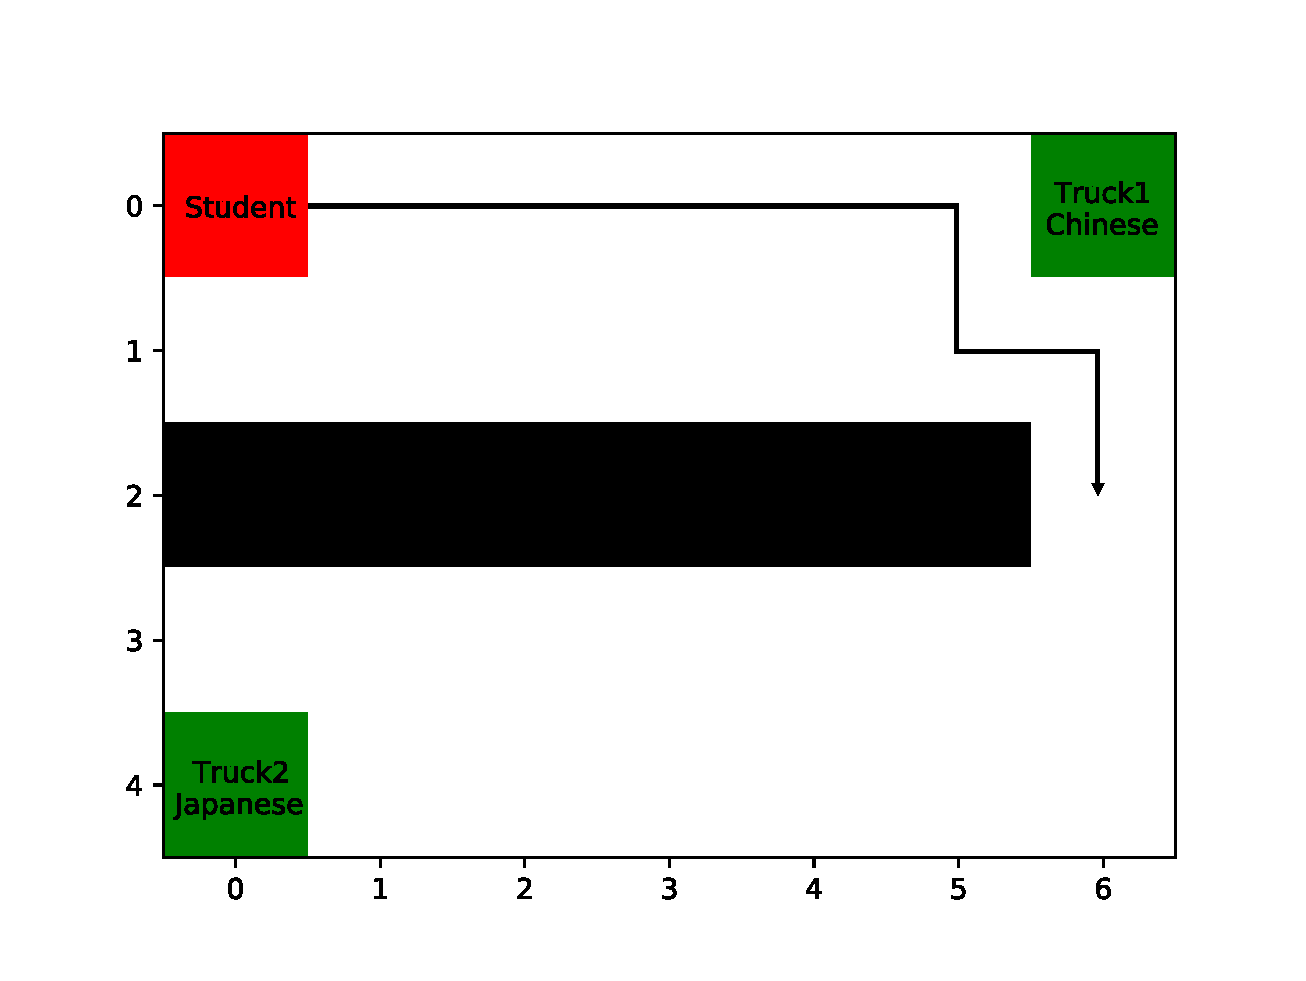
\includegraphics[scale=0.48]{./ex_env2.pdf}
    \caption{行動情報と発話情報が影響を与え合う場面}
    \label{fig:ex_env2}
  \end{center}
\end{figure}
また,Truck1とTruck2のどちらを望んでいるかを特定することができない曖昧な発話情報を行動情報によって補完することもある.MIoM SCAINは,発話情報による行動情報の解釈の変化や行動情報による発話情報の解釈の変化を捉え,行動情報と発話情報の相互作用を推定に反映することでUIoM SCAINの推定結果を上回ったと考えられる.MIoM SCAINの推定により,信念と欲求の推定において行動情報と発話情報を両方用いることが有効であると考えられる.

\par
また,本実験では3つの推定システムにおいて欲求推定の相関が信念推定の相関より強いことが示された.そこで本実験で用いた3つの推定システムにおいて欲求推定が信念推定よりも強い相関を示した要因を考える.実験参加者による推定結果を分析したところ,欲求推定では行動情報と発話情報の両方が大きく影響していたが,信念推定では発話情報の影響が大きいことがわかった.例えば,図\ref{fig:ex_env3}に示すように,Truck1は観測しているがTruck2を観測していない状況でTruck1からは遠ざかりTruck2に向かう状況を考える.
\begin{figure}[htbp]
  \begin{center}
    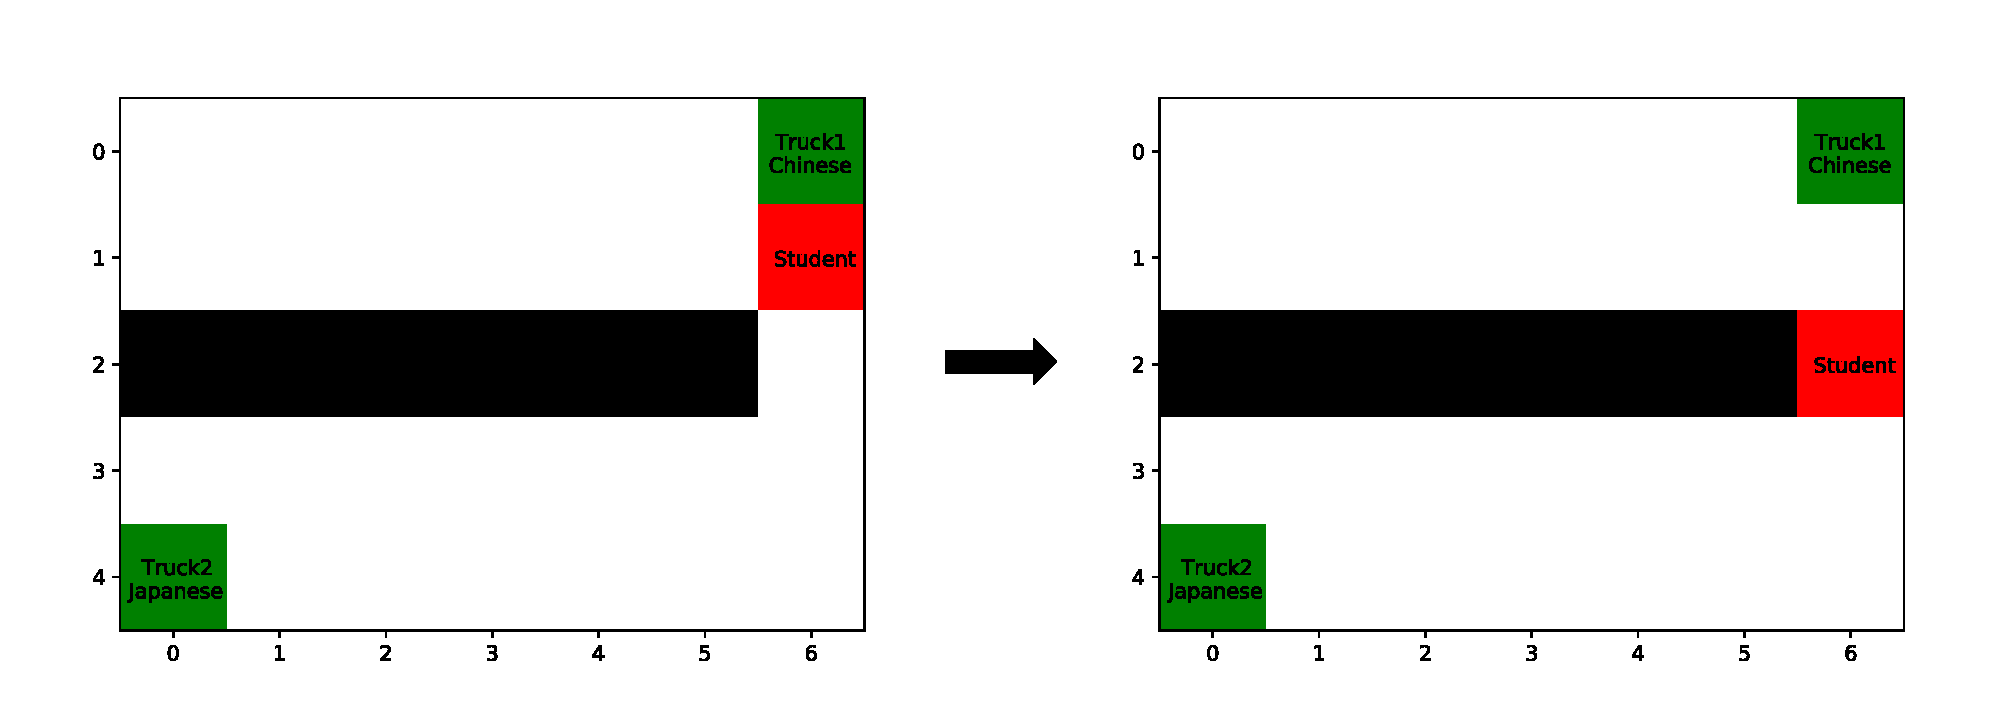
\includegraphics[scale=0.48]{./ex_env3.pdf}
    \caption{学生がTruck1を通過した場面}
    \label{fig:ex_env3}
  \end{center}
\end{figure}
この時,Truck2に向かっているという行動情報は信念の推定に活用することは困難であり,Truck1での食事よりもTruck2での食事を好んでいる可能性が高いという欲求の推定にのみ大きく影響することが考えられる.そのため,実験参加者による信念の推定では発話情報からの影響が大きくなったと考えられる.
しかし発話情報は欲求を問うものが多かったため,発話情報が信念推定に大きな影響を与えることができても,信念の正確な推定に寄与することが困難であったと考える.本実験では,表\ref{tab:q_a}の応答を発話情報として採用している.表\ref{tab:q_a}からわかるように,発話情報は欲求に関する内容である.そのため,発話情報は信念推定および欲求推定に大きい影響を与え,欲求推定の性能向上を寄与することができても,信念推定の性能向上に寄与することはできないと考える.このような理由から,信念推定において信念を問う発話情報を増やすことが有効であると考えられる.

\chapter{今後の課題}

\section{実世界情報による心的状態の推定}
本実験では,人工的なシミュレーションにおける人間の散策行動と人間の発話文から信念と欲求を推定している.散策行動は上,下,左,右の4方向への移動とし,人間の発話文は事前に設定した応答群の中から選択されており,特定の条件における推定を行っている.しかし実世界では,散策行動や人間の発話文は多種多様であり,意図しない散策行動や人間の発話文が生じることも少なくない.今後はVR機器を使用し,実際に人間に散策行動および対話をさせることで,より実世界に似た状況における散策行動情報および人間の発話情報を取得し,人間の信念や欲求の推定に活用するためにMIoM SCAINを拡張する.

\section{人間の発話情報の検討}
% 本実験では,行動$a_t$および発話$u_t$をそれぞれの生起確率$P(a_t)$,$P(u_t)$に変換した.$P(a_t)$は$k$番目のパーティクルが持つ信念$b_t^k$と欲求$d^k$から行動$a_t$が起こる確率として定義した.$P(a_t)$は,信念$b_t^k$と欲求$d$の関係と学生と屋台との距離を基に計算を行っている.

% 埋め込みモデルの検討
% 発話の重要後抽出
% 文章扱い
\par
実験参加者による信念と欲求の推定では散策行動情報よりも人間の発話情報を重視する傾向が見られた.そこで人間の発話情報の検討をすることがMIoM SCAINにおける信念と欲求の推定結果の向上に繋がると考えられる.MIoM SCAINにより信念および欲求を推定するにあたり,人間の発話内容の検討,人間の発話文の推定への活用方法の検討および人間の発話文$u_t$の生起確率$P(u_t)$の計算方法の検討が必要である.

\par
最初に人間の発話内容の検討について考える.本実験では,人間の発話内容として表\ref{tab:q_a}に示す学生の応答内容を採用した.しかし,それらはいずれも欲求に関する内容であるため,欲求の推定に影響を与えることができても信念の推定に影響を与えることが困難であった.また,実世界では条件や制約は存在せず,人間の発話内容は多種多様である.これらの問題を解決するには,人間の発話内容の検討が必要である.人間の発話内容に関して,欲求だけでなく信念に関する発話文を促す質問を提示する機構をMIoM SCAINに搭載することが必要であると考える.信念に関する発話文を促す質問を提示する機構をMIoM SCAINに搭載することで,信念に関する発話情報を取り入れることができるだけでなく,多種多様な人間の発話文を制御することが可能となる.

\par
次に人間の発話文の推定への活用方法の検討について考える.現時点におけるMIoM SCAINでは人間の発話文が観測された場合,それを単語レベルに分解し,単語ごとに生起確率を求める.例えば,``I want to eat rice.''という人間の発話文が観測された時,``I'',``want'',``to'',``eat'',``rice''の単語レベルに分解され,それぞれの単語ごとの生起確率が計算される.しかし,例えば"to"はこの文における重要度が低く,信念や欲求の推定に大きな影響を与えることがないことが予想される.また,信念や欲求の推定に逆効果をもたらす単語が推定に反映されてしまう場合も考えられる.これらの問題を解決するには,人間の発話文の推定への活用方法の検討が必要である.そこで文の重要語抽出手法の適用が考えられる.文の重要語抽出手法を用い,信念や欲求の推定に大きな影響を与える単語を抽出し,生起確率を計算し推定に活用することで,発話文による信念および欲求の推定を実現することができる.

\par
最後に人間の発話文の生起確率の計算方法の検討について考える.MIoM SCAINでは,人間の発話$u_t$をWord2Vecにより分散表現に変換した後,信念$b_t$と欲求$d$との類似度を基に生起確率$P(u_t)$に変換する.しかし単語同士の類似度比較では不十分な場合がある.例えば``Japanese food''と``rice''の類似度を計算する場合を考える.Word2vecでは1単語同士の類似度を計算することは可能だが,この場合のような2単語と1単語の類似度計算を行うことができない.その結果,``Japanese''と``rice''の類似度を計算することになる.しかし,``Japanese''のみでは食事に関する意味が損なわれてしまい,人間が行う類似度比較とは異なることが考えられる.この問題を解決するためには,単語埋め込みモデルの検討が必要である.単語数の異なるテキスト間の類似度を計算することができる単語埋め込みモデルを使用することにより,人間が行う類似度比較に近づけることができる.したがって単語埋め込みモデルの検討により,人間の発話文の生起確率の計算方法を改善することができると考える.


\section{対話システムの発話生成}
% 推定に有利な発話を促す発話生成
% 推定結果を考慮した発話生成
% 発話生成のタイミング

\par
MIoM SCAINは人間の散策行動情報と人間の発話情報を活用した信念と欲求の推定に止まっていた.しかしMIoM SCAINにおける最終目標は,信念や欲求を考慮した対話を行うことである.そこで,推定した信念と欲求を考慮し,MIoM SCAINが発話文を生成する機構を取り入れることが必要である.この機構により,人間の信念と欲求を考慮した発話を生成することで,対話において人間に与える不自然さやストレスを軽減することができ,使いやすい対話システムの実現へ近づくことができると考える.また,この機構により人間の信念と欲求を考慮したタイミングで発話を提示することが可能となる.その結果,発話の内容だけでなく発話のタイミングによっても,対話において人間に与える不自然さやストレスを軽減することができると考える.

\par
また,信念と欲求の推定に大きな影響を与える人間の発話を促す発話を生成することも重要である.今後,より実践的な状況における散策行動情報と人間の発話情報から信念と欲求を推定するにあたり,多種多様な人間の発話が観測されることが予想される.MIoM SCAINはランダムな発話生成を行うのではなく,人間の発話に条件を設けたり,制約をかけることができる発話を生成することが必要であると考える.

\chapter{結論}
本論文では,MIoM SCAINによりマルチモーダルな心的状態推定について検討した.実験の結果,行動情報と発話情報の両方を心的状態の推定に用いることが有効であることを示した.今後の展望としては,より実世界に近い環境設定や三次元の行動および多種多様な発話を扱えるようにMIoM SCAINを拡張したいと考えている.

%%
%%

%
% 謝辞
%
\chapter*{謝辞}
\addcontentsline{toc}{chapter}{謝辞}
\baselineskip = 20pt

\begin{verbatimtab}
	本研究を進めるにあたり、研究の機会及び貴重なご意見を頂きました、
			慶應義塾大学理工学部 今井 倫太 教授
に深く感謝致します。


	論文の査読をして頂き、細部にわたって御意見を頂きました
			理工学研究科博士課程2年 福地 庸介 氏
			理工学部研究員 前川知行 氏
に厚く御礼申し上げます。

  
	実験に御協力頂いた被験者の方々に心より御礼申し上げます。



最後に日頃から御指導、御協力下さいました今井研究室の皆様に心より感謝いたします。


							令和3年1月
\end{verbatimtab}

% \begin{verbatimtab}
% 	本研究を進めるにあたり、研究の機会及び貴重なご意見を頂きました、
% 			慶應義塾大学理工学部 今井 倫太 准教授
% 			慶應義塾大学理工学部 大澤 博隆 助教
% に深く感謝致します。


% 	論文の査読をして頂き、細部にわたって御意見を頂きました
% 			理工学部研究科修士課程1年 尾形 正泰 氏
% に厚く御礼申し上げます。

%   
% 	実験に御協力頂いた被験者の方々に心より御礼申し上げます。



% 最後に日頃から御指導、御協力下さいました今井研究室の皆様に心より感謝いたします。


% 							平成24年1月
% \end{verbatimtab}
    %謝辞

\bibliography{reference}     %参考文献

\end{document}
